% ****** Start of file apssamp.tex ******
%
%   This file is part of the APS files in the REVTeX 4.2 distribution.
%   Version 4.2a of REVTeX, December 2014
%
%   Copyright (c) 2014 The American Physical Society.
%
%   See the REVTeX 4 README file for restrictions and more information.
%
% TeX'ing this file requires that you have AMS-LaTeX 2.0 installed
% as well as the rest of the prerequisites for REVTeX 4.2
%
% See the REVTeX 4 README file
% It also requires running BibTeX. The commands are as follows:
%
%  1)  latex apssamp.tex
%  2)  bibtex apssamp
%  3)  latex apssamp.tex
%  4)  latex apssamp.tex
%
\documentclass[%
 reprint,
%superscriptaddress,
%groupedaddress,
%unsortedaddress,
%runinaddress,
%frontmatterverbose, 
%preprint,
%preprintnumbers,
%nofootinbib,
%nobibnotes,
%bibnotes,
 amsmath,amssymb,
 aps
%pra,
%prb,
%rmp,
%prstab,
%prstper,
%floatfix,
]{revtex4-2}

\usepackage{bm}

\usepackage{caption}
\usepackage{subcaption}
\usepackage{mathtools}
\usepackage{graphicx}% Include figure files
\usepackage{dcolumn}% Align table columns on decimal point
\usepackage{bm}% bold math
%\usepackage{hyperref}% add hypertext capabilities
%\usepackage[mathlines]{lineno}% Enable numbering of text and display math
%\linenumbers\relax % Commence numbering lines
\usepackage{todonotes}

%\usepackage[showframe,%Uncomment any one of the following lines to test 
%%scale=0.7, marginratio={1:1, 2:3}, ignoreall,% default settings
%%text={7in,10in},centering,
%%margin=1.5in,
%%total={6.5in,8.75in}, top=1.2in, left=0.9in, includefoot,
%%height=10in,a5paper,hmargin={3cm,0.8in},
%]{geometry}

\begin{document}

\preprint{APS/123-QED}

\title{High-temperature spectral control and optimization}% Force line breaks with \\
%\thanks{A footnote to the article title}%

\author{William Li}

 \email{wfli@mit.edu}


\date{December 2021}% It is always \today, today,
             %  but any date may be explicitly specified

\begin{abstract}
Nanophotonic structures can be designed to manipulate the emission spectrum of high-temperature materials. This has direct application to lighting, in which there is generally a mismatch between the frequency range detectable by the human eye and the emitted spectrum of the light source \cite{DOE}. This leads to luminous inefficiencies that can be remedied by nanophotonics. Because of the reciprocal relation between thermal emission and absorption, the same problems arise in thermophotovoltaic conversion \cite{shockley}, for which nanophotonic structures can again assist to improve the conversion efficiency. 

In this work, we provide a review of the literature in tailoring high-temperature thermal emission and absorption with nanophotonics, with a focus on the work done by \cite{ilic} on tailoring high-temperature radiation via a cold-side needle-optimized nanophotonic interference system. We use Meep \cite{meep} to reproduce the theoretical and experimental results in \cite{ilic}. We extend the work by formulating a density-based adjoint optimization scheme \cite{adjoint} for cold-side nanophotonic radiation tailoring. For normal emission with a 5-micron 1-d design region, our adjoint optimization scheme achieves $21\%$ luminous efficiency.
\end{abstract}

%\keywords{Suggested keywords}%Use showkeys class option if keyword
                              %display desired
\maketitle

%\tableofcontents

\section{A review of nanophotonics in high-temperature thermal radiation spectral control}


\subsection{Introduction}
In this section, we provide an overview of the topics and recent in high-temperature control. We go into incandescent lighting and infrared sensing, solar thermovoltaics, metallic and dielectric nanostructures, topological transitions, and cold-side nanophotonic tailoring. Due to the reciprocal relation of absorptivity and emissivity from Kirchhoff's law of thermal radiation, much of the work in the different applications of high-temperature spectral control can be applied to each other. Kirchhoff's law says that, for an arbitrary opaque body, the emissivity equals the absorptivity. Tuning a thermal emitter to emit more at a certain frequency means that we have also made an absorber that absorbs more at that frequency.


\subsection{Incandescent lighting and nondispersive infrared sensing}
Incandescent bulbs produce light by thermal radiation from a high-temperature metal filament (for example, tungsten). A major problem with using incandescence as a light source is the luminous inefficiency. Much of the energy emitted by incandescent bulbs is in the infrared region, emitted at wavelengths invisible to the human eye. For modern commercial purposes, this means other lighting methods (e.g. LED, fluorescence) have steadily been replacing incandescent lights from the market. 

By designing the lighting system to have some sort of spectral control that selects for the visible range, we can greatly increase the efficiency of incandescent lighting. One way of doing this is to recycle the energy from infrared radiation \cite{heat_mirror}. In other words, design a system that will reflect infrared light back to the source, where it is reabsorbed and used to emit more light. Such a system would then only let out light in the visible range, increasing its luminous efficiency. Other work for lighting has been done on improving the emitter itself, such as femtosecond laser blackening to enhance the emission efficiency of tungsten \cite{femto}.

There has also been work on using interference stacks for cold-side thermal spectrum tailoring of incandescent lighting \cite{ilic, view_factor_1, view_factor_2}, which will be the biggest focus for this paper. 

Another application of spectral control is in the detection of gas concentrations through a technique called nondispersive infrared sensing (NDIR). Nondispersive infrared sensing detects gas concentrations through analyzing the attenuation of wavelengths by the gas. The nondispersive part means that there is no dispersive element to separate different frequencies \cite{gas_detection}. Because NDIR only uses midinfrared thermal emission (due to the absorption spectra of gases), gas detection can be made more efficient by controlling thermal emitters to emit in narrowband infrared frequencies.

\subsection{Solar thermovoltaics}
The most common existing approaches to generate power from sunlight are photovolatics and solar-thermal \cite{lenert}. Photovoltaic solar cells work by using sunlight to directly excite the electron-hole pair frequencies in a bandgap of a semiconductor to generate energy. The most common photovoltaic design uses a silicon p-n junction. A p-n junction is a boundary between a positive (`p'-type) semiconductor material and a negative (`n'-type) semiconductor material. The p-side is hole-rich, and the n-side is electron-rich. p-type and n-type materials are made by doping. When put together, a neutral region forms at the boundary, called the p-n junction. Under ordinary conditions, p-n junctions only allow electrons to flow from the n-side to the p-side (``foward direction") \cite{famu}. Sunlight makes electrical current by exciting electrons on the p-side and sending them through an external circuit to the n-side, where they return to the p-side in the forward direction. 
\begin{figure}
\centering
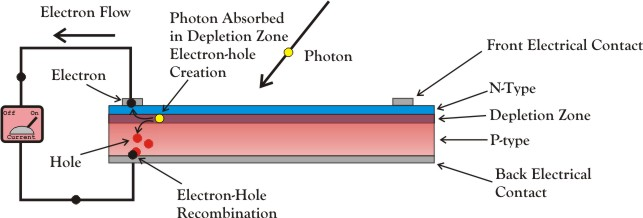
\includegraphics[width=0.8\linewidth]{solarcellW.jpg}
\caption{An illustration of a photovoltaic solar cell with a single p-n junction. Figure from \cite{photovolt}.}\label{junction}
\end{figure} Solar energy is extracted from the external circuit. This is illustrated in Figure \ref{junction}.

With single p-n junction solar cells, the efficiency is capped by the Shockley-Queisser limit \cite{shockley} because electron-hole pairs in a semiconductor are only excited by a relatively narrow range of frequencies. In general, photovoltaic efficiency, or the portion of sunlight energy that can be converted into electricity, is limited by the mismatch between the solar spectrum and the semiconductor's absorption profile. Photons with energy below the semiconductor's electronic bandgap are not absorbed, and photons above the bandgap don't generate significant energy. The Shockley-Queisser limit for single-junction cells is 41\%. But if spectrum matching was solved, i.e. if solar radiation only came in the desired frequency range, then single-junction cells would only be limited by the second law of thermodynamics, and so approach efficiencies of 95\% \cite{shanhui}. 

The other main existing approach to generate power from sunlight is solar-thermal. Solar-thermal systems work by using sunlight to run a heat engine. However, this is not a good approach for small heat engines in which irreversible processes cause significant energy loss \cite{lenert}.

This leads to the area of {\it solar thermophotovoltaics}, a hybrid system that matches solar radiation with the photovoltaic bandgap using a high-temperature absorber-emitter. This concept was first proposed in the 1970s \cite{swanson} (see Figure \ref{swanson_fig}). Solar radiation shines onto the absorber-emitter, heating it and causing it to emit thermal radiation, which can in principle be tailored to the desired frequencies. The thermal radiation is then absorbed by the semiconductor. The absorber-emitter is designed to convert the entire solar spectrum into frequencies that work with the photovoltaic bandgap. In theory, an ideal absorber-emitter intermediate couppled with a single-junction cell could have 85\% efficiency \cite{harder}. 

However, solar thermophotovoltaics have been difficult to implement in practice because absorber-emitter materials that work well at high temperatures (e.g. tungsten and graphite) do not do much for spectral control. One recent development in the area was the work by \cite{lenert} that demonstrates a one-dimensional photonic crystal of Si and SiO2 at 1300 K to achieve a sunlight-to-electricity efficiency of 3.2\%. Although this is still far from the efficiency of modern single-junction solar cells (around 30\% \cite{conversion_eff}), it is progress toward the theoretical promises of thermophotovoltaics. 

The work by \cite{lenert} uses a 1-dimensional photonic crystal as the absorber-emitter. Other structures that have been used as the intermediate absorber-emitter include bulk emitters, selective emitters, 2-dimensional photonic crystals, and multilayer stacks \cite{tpv_review}. Moreover, thermophotovoltaics has application to radioisotope fuel and chemical decay as well in addition to its use in solar energy conversion \cite{tpv_review}.

\begin{figure}
\centering
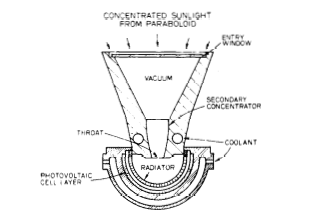
\includegraphics[width=0.8\linewidth]{swanson.PNG}
\caption{The proposed thermophotovoltaic design from Swanson's original paper \cite{swanson}.}\label{swanson_fig}
\end{figure} 

\begin{figure}
\centering
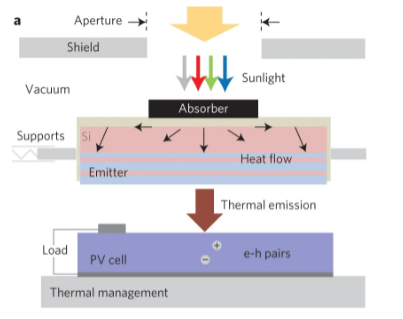
\includegraphics[width=0.8\linewidth]{stpv_schematic.png}
\caption{A schematic from \cite{lenert} for converting sunlight into thermal emission then electric power through a solar thermophotovoltaic system.}\label{lenert_fig}
\end{figure} 
\subsection{Metallic and dielectric nanostructures for thermal emission control}
In this subsection, we discuss the ways in which thermal emission control is implemented through the choice of materials and design possibilities. Compared to the previous two subsections, this subsection has a bigger focus on the design rather than the application.

Broadly, thermal emission control can be done through either metal emitters or dielectric emitters. There are advantages and disadvantages to each. Dielectrics are better at spectral control, but the mechanisms by which they work fail at temperatures higher than 700 or 800 K \cite{nanostructures}.

Within the subgroup of metal emitters, there are metallic nanostructures and metallic metamaterials. Metallic nanostructures include things like photonic crystals \cite{polycrystalline} and microcavity arrays \cite{microcavity}. Metal photonic crystals control emission frequencies their photonic bandgap and resonant modes at the photonic band edges. Microcavity arrays control emission frequencies through their confined modes inside the microcavities \cite{nanostructures}. By choosing a metal like tungsten or tantalum, very high temperatures can be reached without degradation. The temperatures required for incandescence, however, can still cause problems \cite{ilic}.

Metal emitters can also be metallic metamaterials. Metallic metamaterials consist of arrays of metals with thin dielectric layers. By designing the metal arrays, the permittivity and permeability of the entire metamaterial can be controlled. Matching the metamaterial impedance $\sqrt{\frac{\mu}{\varepsilon}}$ to the free space impedance allows metamaterials to achieve perfect absorption at given frequencies \cite{nanostructures}. Other work done with metallic metamaterials uses topological transitions to control the thermal emission spectrum. For example, the work in uses a tungsten-HfO2 metamaterial to selectively enhance and suppress thermal emission. A significant advantage of metamaterials is the lack of angle-dependence \cite{topological}.

Metals have a drawback in that free carrier absorption leads to broadband emission, which makes spectral control difficult. Dielectric nanostructures don't have this problem, as materials like undoped Si and GaAs are transparent for most frequencies. To get emission out of them, we can use the Restrahlen band or multiple quantum wells \cite{nanostructures}.


\subsection{Cold-side nanophotonic tailoring}
Finally, we discuss cold-side nanophotonic tailoring, which will be the focus for the rest of this paper. The cold-side tailoring the actual high-temeprature emitter or absorber is not modified. This allows for extremely high temperatures because we no longer have to worry about the heat degrading the nanophotonic patterning. Instead, the nanophotonic structures are built around the high-temperature emitter, so the patterned structures themselves remain cool (thus ``cold-side"). An example of this setup is in Figure \ref{fig:test} from \cite{ilic}. The work by \cite{ilic} uses a bare tungsten filament as the high-temperature emitter and a multilayered dielectric stack as the cold-side structure. 

In \cite{ilic}, the cold-side nanophotonic structure is characterized by three quantities: its transmittance spectrum $T(\lambda)$, its reflectance spectrum $R(\lambda)$, and the view factor $F$. The view factor is defined as the proportion of energy leaving the emitter that is intercepted by the nanophotonic structure. The work in \cite{ilic} assumes a high view factor (close to 1, meaning nearly all of the light is intercepted by the nanophotonics) and then optimizes the structure to get the desired transmittance and reflectance spectra.

In real-world lighting however, view factors are important, and we generally cannot assume them to work in our favor. More recent work deals with this. The work in \cite{view_factor_1} combines a cold-side structure with a {\it selective} emitter to overcome the view factor problem. Here, they do both cold-side and hot-side tungsten coating with HfO2. HfO2 coating increases the effective emissivity in the visible spectrum, giving this design more power over the bare tungsten plus interference stack used in \cite{ilic}. Even more recent work investigates adding specular side reflectors between the emitter and the cold-side structure to increase the effective view factor \cite{view_factor_2} (see figure \ref{side_refl} for a schematic).

\begin{figure}
    \centering
    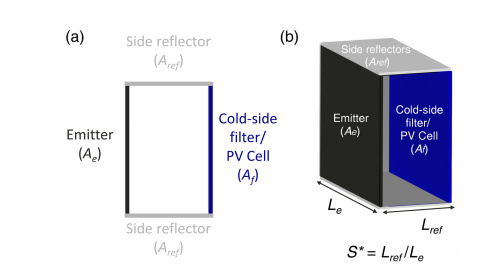
\includegraphics[width=.7\linewidth]{cold_side_specular.jpeg}
    \caption{A schematic from \cite{view_factor_2} of their side reflector design to enhance the view factor for cold-side thermal emission tailoring.}
    \label{side_refl}
\end{figure}
\section{Reproduction of cold-side nanophotonic tailoring} \label{reproduction}

In this section, we reproduce the theoretical and experimental results of \cite{ilic} using Meep \cite{meep}. Meep is an open-source software package that performs electromagnetic simulations using the finite-difference time-domain (FDTD) method.

\subsection{Notation}
We will be using $\epsilon(\lambda, \theta)$ for directional spectral emissivity or emittance. We use $\epsilon(\lambda)$ for the {\it hemispherical} spectral emissivity, where \begin{equation}
\epsilon(\lambda) = \frac{\int_0^{\pi/2}\epsilon(\lambda, \theta)\sin\theta\cos\theta d\theta}{\int_0 ^ \pi/2 \sin\theta\cos\theta d\theta}.
\end{equation} We're always talking about hemispherical spectral emissivity when $\theta$ is not indicated. This is also true for the reflectance $R$ and the transmittance $T$ when we discuss those. Because epsilon is also used to indicate dielectric dispersion, we indicate the dielectric dispersion of our materials with the inverted-3 form of epsilon $\varepsilon(\lambda)$.
\subsection{Setup}

\begin{figure}
\centering
\begin{subfigure}{.25\textwidth}
  \centering
  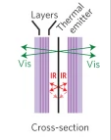
\includegraphics[width=.8\linewidth]{setup.PNG}
  \label{fig:sub1}
\end{subfigure}%
\begin{subfigure}{.25\textwidth}
  \centering
  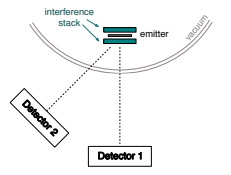
\includegraphics[width=.8\linewidth]{experimental_setup.PNG}
  \label{fig:sub2}
\end{subfigure}
\caption{Figures from \cite{ilic} showing the setup of cold-side nanophotonic tailoring.}
\label{fig:test}
\end{figure}

In cold-side nanophotonic tailoring, the high-temperature incandescent emitter is a plain tungsten filament. The nanophotonic interference system is built around it to reflect infrared light and transmit visible light. The interference system consists of two identical one-dimensional layered stacks of dielectric materials. 

\subsection{Effective emissivity and luminous efficiency}
The primary goal of \cite{ilic} is to design the interference stacks in the above setup to optimize the luminous efficiency \begin{equation}\eta = \frac{\int_0^{\infty} P(T, \lambda) V^*(\lambda) d\lambda}{\int_0^\infty P(T, \lambda) d\lambda}.\end{equation}

$P(T, \lambda)$ is the hemispherical spectral emissive power of the emitter at temperature $T$. $V^*(\lambda)$ is the photopic spectral luminous efficiency function. It is a measure of the sensitivity of the human eye at day to different wavelengths of light. $\eta$ therefore captures the proportion of emitted power that we can see.

We can further write $P(T, \lambda)$ in terms of Planck's blackbody spectra radiance function $B_\lambda (\lambda, T)$ and the effective emissivity $\epsilon_{\text{eff}}(\lambda)$ of our emitter-interference structure. This gives us \begin{equation}\label{eq:extended}\boxed{\eta = \frac{\int_0^{\infty} \epsilon_{\text{eff}} (\lambda, T) B_\lambda (\lambda, T) V^*(\lambda) d\lambda}{\int_0^{\infty} \epsilon_{\text{eff}} (\lambda, T) B_\lambda (\lambda, T) d\lambda}}.\end{equation}

From the supplementary material of \cite{ilic}, we can write the effective emissivity in terms of the tungsten emissivity $\epsilon(T, \lambda)$ as 

\begin{equation} \label{epseff}
\begin{multlined}
\epsilon_{\text{eff}}(\lambda, T) = \epsilon(\lambda, T)\cdot \bigg [ \frac{F \cdot T(\lambda)}{1 - F^2 \cdot R(\lambda)\cdot(1-\epsilon(\lambda))} \\+ \frac{(1-F)\cdot(1+F\cdot R(\lambda))}{1 - F^2 \cdot R(\lambda) \cdot (1-\epsilon(\lambda))} \bigg].
\end{multlined}
\end{equation}
Here $T$ is the transmittance and $R$ is the reflectance of the interference stack. $F$ is the view factor of the system, which equals the proportion of energy leaving the emitter that is directly intercepted by the stack. We assume that the planar dimensions of the system are large compared to the dimensions normal to the plane, so little radiation escapes around the edges, implying a view factor close to $1$ (like in \cite{ilic}, we will take $F$ to be $0.95$).

We obtain the expression and tabulated values for the photopic spectral luminous efficiency function $V^*(\lambda) = 1.55 L(\lambda) + M(\lambda)$ from \cite{sharpe}, where $L(\lambda)$ and $M(\lambda)$ are the Stockman and Sharpe cone fundamentals.

\begin{figure}
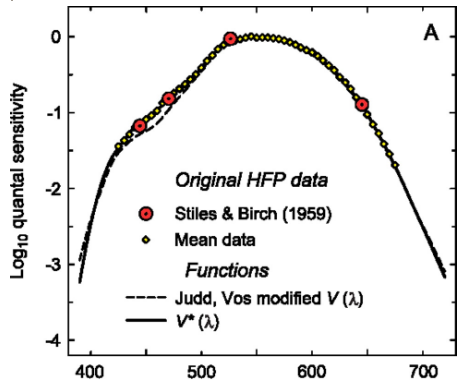
\includegraphics[width=.8\linewidth]{sharpe.PNG}

\caption{The fit of the photopic luminosity function $V^*(\lambda)$ (continuous line) to experimental measurements of quantal sensitivity. Figure from \cite{sharpe}.}
\end{figure}

We use tabulated values for tungsten high-temperature normal spectral emittance $\epsilon(\lambda, \theta=\pi/2, T=3000 K)$ from \cite{touloukian}. Values in the table were available for 2800 K and 3100 K, and we use linear interpolation to find the value at 3000 K. Because absorptivity equals emissivity, we can also find normal-incident reflectivity of the high-temperature tungsten $R$ as $R(\lambda) = 1 - \epsilon(\lambda)$. We will use this to fit the Drude-Lorentz model below.

To obtain the emittance at an angle (which we need for the hemispherical emittance $\epsilon (\lambda)$), we first find the complex permittivity at 3000 K by fitting a Lorentz-Drude model with four Lorentz terms. We use the form of the equation quoted in \cite{minissale}: \begin{equation}\begin{multlined}\varepsilon(\lambda = 2\pi/\omega, T=3000K) = 1-\frac{f_0 \omega_p^2}{\omega(\omega-i\Gamma_0)} \\+ \sum_{i=1}^4 \frac{f_i \omega_p^2}{\omega_i^2 - \omega^2 + i\omega\Gamma_i},\end{multlined}\end{equation}
where we tune $\omega_p$ and each $f_i, \Gamma_i$. From $\varepsilon$, we can compute the modeled normal reflectivty as \begin{equation}R^*(\lambda) = \left |\frac{1-\sqrt{\varepsilon}}{1+\sqrt{\varepsilon}} \right |^2.\end{equation}

We tune our parameters to minimize the proportional error in reflectivity $\frac{|R^*(\lambda) - R(\lambda)|}{R(\lambda)}$ summed over all available wavelengths $\lambda$. Fitting is performed using global optimization algorithm DIRECT-L implemented in NLopt \cite{nlopt, direct-l}. Our tuned parameters are provided in Table~\ref{Tab:Tcr}. 

\begin{table}[ht]
\caption{Tuned values of the Lorentz-Drude model parameters to fit tungsten reflectance at 3000 K. $\omega_i, \omega_p,$ and $\Gamma_i$ are in eV. $f_i$ is dimensionless.}
\centering
  \begin{tabular}{l l l l l l}
    Oscillator  & i & $\omega_i$ & $f_i$ & $\Gamma_i$ &$\omega_p$\\
    \hline
     & & & & & 10.00\\
    Drude      & 0 & & 3.35 &  6.67  &            \\
    Lorentz      & 1 & 13.11& 9.79&   18.73 &            \\
    Lorentz        & 2& 11.11& 8.89 &  0.47 &          \\
    Lorentz        & 3& 10.12& 16.68 &  19.97  &          \\
    Lorentz        & 4& 10.00& 10.00 &  10.00 &           \\
  \end{tabular}
  \label{Tab:Tcr}
\end{table}

\begin{figure}
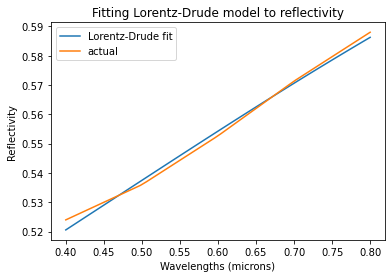
\includegraphics[width=.9\linewidth]{LD.PNG}

\caption{Globally optimized fit of the Drude-Lorentz model to tabulated data for a tungsten emitter at 3000 K. The tabulated data is of a 99.9\% tungsten sample from Carbide Specialty Co., polished and washed.}
\end{figure}
Once we have $\varepsilon(\lambda)$, we compute the angular reflectivity using the Fresnel equations, taking the average of reflectivity from $s$ and $p$ polarized light because we have unpolarized thermal radiation. In the limit of opaque materials (which we have), absorptivity is $1$ minus reflectivity. From Kirchoff's law, absorptivity equals emissivity, giving us $\epsilon(\lambda,\theta)$ for all angles $\theta$. 

\subsection{Reproduction of experimental angular reflectance spectrum}
The two primary results of \cite{ilic} are their needle-optimized 4-material 300-layer design and their fabricated proof-of-concept 2-material 90-layer structure. The four materials used are SiO2, Al2O3, Ta2O5, and TiO2. We used the permittivities for these materials at 610 nm without modeling dispersion relation or loss. 
\begin{figure}
\centering
\begin{subfigure}{.3\textwidth}
  \centering
  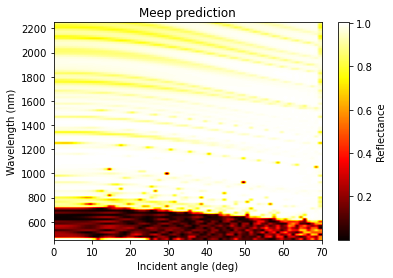
\includegraphics[width=1.\linewidth]{meep_fig_3_colorbar.PNG}
  \label{fig:sub1}
\end{subfigure}%
\begin{subfigure}{.3\textwidth}
  \centering
  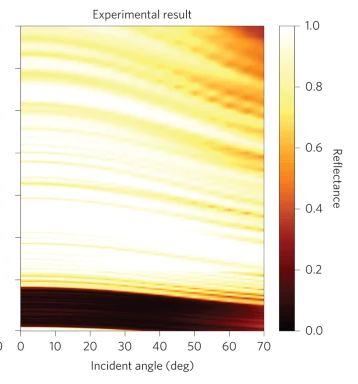
\includegraphics[width=.85\linewidth]{actual_fig_3.PNG}
  \label{fig:sub2}
\end{subfigure}
\caption{Side-by-side comparison of our computed reflectance spectra of the 90-layer fabricated stack (left) with the experimental data from \cite{ilic} (right). The most important part of these images is the high transmittance in the visible-light region (approximately 380 to 700 nm) and the almost complete reflectance in the infrared region of the spectrum. This mechanism is how the interference stacks increase luminous efficiency.} 
\label{fig_3_reproduce}
\end{figure}
Using the 90-layer fabrication specifications in the supplementary information of \cite{ilic}, we simulate the reflectance spectrum over a wide range of angles using the procedure laid out in \cite{meep_tutorial}. Following the advice in \cite{meep_tutorial}, we use narrowband sources to avoid glancing angle effects in our simulations. To do so, we ran separate simulations for each angle and wavelength. For computational efficiency, we only simulated $E_z$-polarized light in our calculations. In figure \ref{fig_3_reproduce} we present our predicted result compared to the experimental measurement in \cite{ilic}.


\subsection{Reproduction of effective emissivities}
In this subsection, we reproduce the claim at the heart of the the work in \cite{ilic}---that the effective emissivities of the optimized and fabricated stacks overlap the photopic luminous efficiency function very well, resulting in high luminous efficiency. To do this, we reproduce the emitted power spectrum for a bare emitter, the fabricated stack, and the optimized stack at 3000 K.  

In other words, we find $\epsilon_{\text{eff}} (\lambda, T) B_\lambda (\lambda, T)$ at $T=3000 K$ for both the fabricated stack and optimized stack and compare them to the power spectrum from a bare emitter $\epsilon(\lambda, T) B_\lambda (\lambda, T)$. From equation \ref{epseff}, we can compute $\epsilon_{\text{eff}}$ as a function of $\epsilon$, $R$, and $T$. $R$ and $T$ are both computed using Meep as in the previous subsection. For all computations, we compute the power spectrum from 400 nm to 2250 nm. Our results are compared side-by-side with the results from \cite{ilic} in figure \ref{fig_2_reproduce}.

\begin{figure}
\centering
\begin{subfigure}{.25\textwidth}
  \centering
  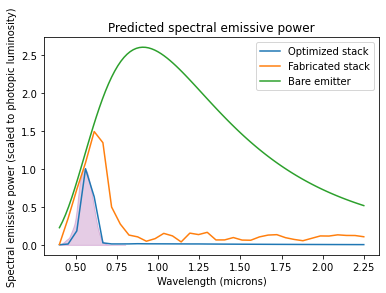
\includegraphics[width=1.\linewidth]{reproduce_fig_2.pn.png}
  
  \label{fig:sub1}
\end{subfigure}%
\begin{subfigure}{.25\textwidth}
  \centering
  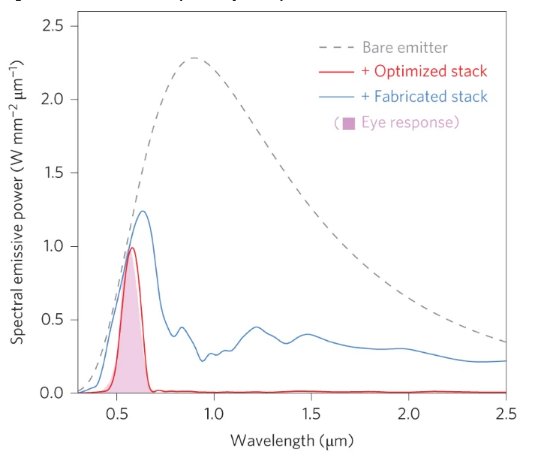
\includegraphics[width=1.\linewidth]{actual_fig_2.png}
  \label{fig:sub2}
\end{subfigure}
\caption{Side-by-side comparison of our computed spectral power (left) with the results from \cite{ilic} (right). The setup is a 3000 K tungsten emitter sandwiched between two interference stacks. On the left, we plot the computed spectral power integrated over a hemisphere from the 300-layer needle-optimized stack (blue), the 90-layer fabricated stack (orange), and a bare tungsten emitter (green). The shaded purple region in our figure represents the photopic luminosity function. On the right is the plot from \cite{ilic}, showing the same things but in different colors.} 
\label{fig_2_reproduce}
\end{figure}

Our plots show agreement with the results in \cite{ilic}. The key takeaway here is that the optimized and fabricated structures are much better aligned with the human eye response than a bare incandescent emitter. From the plots, we can see that the peak-amplitude wavelength of emission is pulled down to match the peak-amplitude wavelength response of the human eye. 

We also compute the luminous efficiencies $\eta$ for the needle-optimized and fabricated stacks. Doing so, we find $\eta_{\text{optimized}} = 65\%$ and $\eta_{\text{fabricated}} = 26\%$. Our value for $\eta_{\text{optimized}}$ is a lot higher than the value reported in \cite{ilic}, which is given at around $40\%$. The work in \cite{ilic} claims that an upper limit on efficiency comes from a blackbody emitter that only emits in the wavelengths visible to the human eye (where $V^*(\lambda) > 0.01$), and they report a value around $40\%$ for this ideal efficiency. When replicating that calculation, we get that as well. 

However, I don't think this bound applies to our situation. The hypothetical blackbody emitter has a disadvantage in that it doesn't tailor the wavelengths {\it within} the range of wavelengths visible to the human eye. From figure \ref{fig_2_reproduce}, we see that is not the case for the optimized emitter. In fact, the optimized emitter appears to have a near-perfect fit to the luminosity function $V^*(\lambda)$ in both \cite{ilic} and our replication. Therefore, we should get around the same answer for $\eta_{\text{optimized}}$ as if we just integrate $V^*(\lambda)$ against itself for the calculation. Indeed, if we do that to compute \begin{equation}\eta_{\text{fit}} = \frac{\int V^*(\lambda)^2}{\int V^*(\lambda)},\end{equation} we get an efficiency of around $70\%$. This matches much more closely to the value we found, $\eta_{\text{optimized}} = 65\%$. As far as I can tell, assuming I didn't make any mistakes in my calculations, the work in \cite{ilic} may have reported a lower value for the efficiency because the higher values didn't appear to fit with their bound.

This concludes our work on reproducing the results in \cite{ilic}. We have gone through the methodology of \cite{ilic} to compute the effective emissivity and luminous efficiency, reproduced the experimentally observed fabricated structure reflectance spectra using Meep, and reproduced the key result of the paper through Meep and the following calculations.

\section{Formulation and demonstration of adjoint optimization for inverse design of cold-side interference stacks}
In this section, we formulate and demonstrate optimization through the adjoint method to inverse-design an interference stack to maximize luminous efficiency $\eta$.
\subsection{Formulation}
To recap, we're looking to maximize the luminous efficiency \begin{equation}\eta = \frac{\int_0^{\infty} P(T, \lambda) V^*(\lambda) d\lambda}{\int_0^\infty P(T, \lambda) d\lambda}.\end{equation}
$\eta$ is thus our objective function.

We operate in the case where $T=3000K$. The emitted power spectrum $P(T=3000 K, \lambda)$ is an implicit function of our interference stack's dielectric profile $\varepsilon(x)$. For example, figure \ref{fig_2_reproduce} is the refractive index profile (square root of the dielectric profile) of the 90-layer fabricated interference stack made by \cite{ilic} that we discussed in the last section.
\begin{figure}
\centering
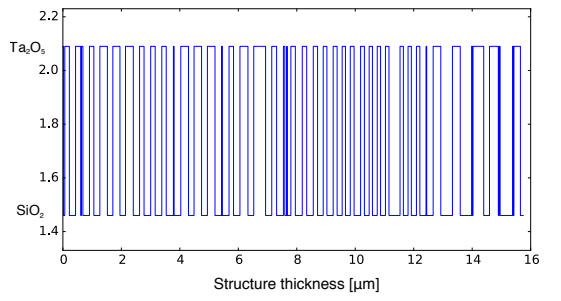
\includegraphics[width=1.\linewidth]{fabricated_stack.PNG}
\caption{The refractive index profile $n = \sqrt{\varepsilon}$ of the fabricated 90-layer 2-material interference stack from \cite{ilic}.} 
\label{fabricated_Stack}
\end{figure}
In order to perform adjoint optimization on the dielectric profile, we need an expression for the optimization gradient $\frac{d \eta}{d\varepsilon(x)}$. Once we have that, we can use our algorithm of choice (gradient descent, Adam optimization \cite{adam}, method of moving asymptotes \cite{mma}, and so on) to find the dielectric profile $\varepsilon(x)$ that maximizes $\eta$. For the rest of this subsection, we discretize the dielectric profile to a vector $\pmb{\varepsilon} = \varepsilon(x)$.

We write Maxwell's equations in discretized form as \begin{equation}
    M(\pmb{\varepsilon}) \pmb{e} = \pmb{s},
\end{equation}
where $\pmb{e}$ is the electromagnetic fields, $\pmb{s}$ is the sources, and $M$ is the linear relationship between the two (Maxwell's equations). $M$ is an explicit function of the dielectric profile $\pmb{\varepsilon}$.

Using the chain rule, we have \begin{equation}
    \frac{d\eta}{d\pmb{\varepsilon}} = \frac{\partial\eta}{\partial \pmb{\varepsilon}} + \frac{\partial \eta}{\partial \pmb{e}} \frac{\partial \pmb{e}}{\partial\pmb{\varepsilon}}.
\end{equation}

Our objective $\eta$ has no explicit dependence on $\pmb{\varepsilon}$, so the first term is $0$. The second term in its current form is difficult to compute due to the costs of differentiating the fields $\pmb{e}$ with respect to $\pmb{\varepsilon}.$ This is because we would need to differentiate Maxwell's equations to get \begin{equation}\label{differentiate} \frac{\partial\pmb{e}}{\partial \pmb{\varepsilon}} =-M^{-1}\frac{\partial M}{\partial \pmb{\varepsilon}} \pmb{e},\end{equation}
and then we would have to find a solution to Maxwell's equations for every element in $\pmb{\varepsilon}$.

Fortunately, this problem can be resolved efficiently with the adjoint method \cite{adjoint}. The key here is that we can expand $\frac{\partial \pmb{e}}{\partial\pmb{\varepsilon}}$ and then take advantage of the associative property in the chain rule to efficiently compute the gradients by multiplying in a less obvious order. 

We expand to get our gradient with respect to $\eta$ \begin{equation} \label{full_adjoint}
   \frac{d\eta}{d\pmb{\varepsilon}} = -\left [\frac{\partial \eta}{\partial \pmb{e}} M^{-1}\right ]\frac{\partial M}{\partial \pmb{\varepsilon}} \pmb{e}.
\end{equation}

Rather than solving for $M^{-1}\frac{\partial M}{\partial \pmb{\varepsilon}} \pmb{e}$ first, we can instead first compute $\frac{\partial \eta}{\partial \pmb{e}} M^{-1}$. This is our {\it adjoint problem}, in which we only have to solve Maxwell's equations once. The rest of the computation is then a straightforward multiplication.

We therefore compute $\frac{d \eta}{d\varepsilon(x)}$ in three steps: first, we use automatic differentiation to compute the gradients of $\eta$ with respect to the electromagnetic fields $e$; then, we use those gradients as the sources to Maxwell's equations in the adjoint problem; finally, we put it all together according to equation \ref{full_adjoint} to get $\frac{d  \eta}{d\varepsilon(x)}$.

Computing $\frac{d\eta}{d \pmb{e}}$ requires differentiating through equations \ref{eq:extended} and \ref{epseff} to get $\frac{d\eta}{d R}$ and $\frac{d\eta}{dT}$. The reflectance $R$ and transmittance $T$ are explicit functions of the fields $\pmb{e}$. In practice, we do all of this with an automatic differentiation package such as autograd \cite{autograd}. 

To summarize our differentiation pipeline, we write out the gradient propagation as \begin{equation}
    \label{full pipeline}
    \boxed{\frac{d \eta}{d \pmb{\varepsilon}} = \left [\frac{\partial \eta}{\partial P}\frac{\partial P}{\partial \epsilon_{\text{eff}}}\left (\frac{\partial \epsilon_{\text{eff}}}{\partial F} \frac{\partial F}{\partial \pmb{e}} + \frac{\partial \epsilon_{\text{eff}}}{\partial T}\frac{\partial T}{\partial \pmb{e}}\right )M^{-1}\right ]\frac{\partial M}{\partial \pmb{\varepsilon}} \pmb{e}},
\end{equation}
where the bracketed part is the adjoint problem.
\subsection{Demonstration}
We demonstrate this optimization on an optimization region $5$ microns thick. By comparison, the fabricated design from \cite{ilic} is around 16 microns thick and the needle-optimized design is 49 microns thick. We do our optimization with Adam \cite{adam}. We constrain our design region's dielectric profile to be within $2.13$ and $5.52$, the dielectric constants of SiO2 and TiO2, which are the lowest and highest permittivity materials used by \cite{ilic}. 

Because of computational costs, we were not able to go that high for a more direct comparison of the methods. Also because of computational costs, we only optimize for the luminous efficiency of normal emission. Again, this means our results are not directly comparable to those of \cite{ilic}. I believe many of these costs can be resolved by a more efficient simulation design---the results I gathered in section \ref{reproduction} were efficiently implemented in 1-dimension, but here I couldn't figure out how to configure the adjoint code to really take advantage of the 1-d structure of the problem.

\begin{figure}
\centering
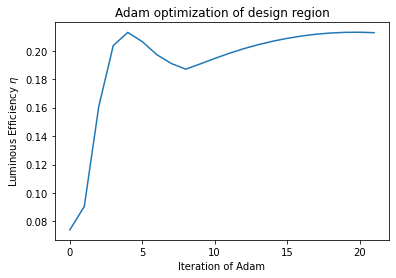
\includegraphics[width=1.\linewidth]{adam_plot.png}
\caption{Our optimization curve for Adam through our adjoint optimization pipeline. Luminous efficiency $\eta$ is plotted on the y-axis, and the number of iterations is plotted on the x-axis. Our design achieves about 21\% luminous efficiency with a 5-micron structure.} 
\label{adam_opt}
\end{figure}
\begin{figure}
\centering
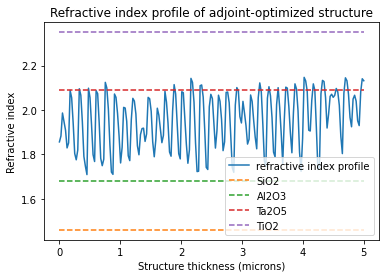
\includegraphics[width=1.\linewidth]{adjoint_opt_struct.png}
\caption{Our adam-optimized dielectric profile with the four materials used by \cite{ilic} in their optimized structure for comparison.} 
\label{adam_struct}
\end{figure}
\begin{figure}
\centering
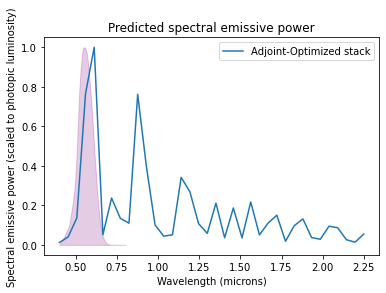
\includegraphics[width=1.\linewidth]{predicted_emissivity.png}
\caption{The normal emitted spectrum of our adjoint-optimized 5-micron design with the photopic luminosity function shaded. Although our design has failed to eliminate the initial bare tungsten emission peak at 0.9 microns, it has made it lower than the photopic luminosity $V^*(\lambda)$ peak at 0.55 microns.} 
\label{adam_struct}
\end{figure}

We show our optimization curve in figure \ref{adam_opt} and our resulting structure in figure \ref{adam_struct}. Our structure achieves a normally-incident luminous efficiency of $21\%$ with a 5-micron design region. As a guideline comparison, the 16-micron fabricated structure from \cite{ilic} achieved a hemispherical luminous efficiency of $26\%$ and the 49-micron needle-optimized structure from \cite{ilic} achieved a hemispherical luminous efficiency of 65\%. As we noted above however, we don't do hemispherical optimization and our structure is thinner than both of the ones discussed in section \ref{reproduction}, so the results are not directly comparable. 

Our results do however show that adjoint optimization holds promise as an alternative optimization scheme for cold-side thermal emission tailoring.
\section{Conclusion}

\subsection{Summary}
We reviewed the topics and literature in nanophotonic spectral control of high-temperature thermal radiation, reproduced the key results in \cite{ilic}, and formulated and demonstrated adjoint optimization for cold-side tailoring of incandescent lighting. 

In our review, we discuss both the applications of tailoring thermal emission spectra (lighting, sensing, thermophotovoltaics) and the nanophotonic designs to achieve spectrum control (metallic nanostructures and metamaterials, all-dielectric photonic crystals, cold-side tailoring). 

In our reproduction of the key results of \cite{ilic}, we work through the components of computing the luminous efficiency $\eta$ and fit the Lorentz-Drude model to find the angular-spectral emissivity of tungsten, reproduce the experimental angular reflectance spectrum of the fabricated design from \cite{ilic} using Meep, and reproduce the key result showing how the power spectrum changes due to the cold-side nanophotonic interference stacks specified by \cite{ilic}. We also note a possible underreporting in their claim of 40\% efficiency for the needle-optimized design that could be because of a misinterpretation of the blackbody limit.

Finally, we formulate an optimization scheme for cold-side tailoring using the adjoint method and we demonstrate our optimization on a 5-micron design region. 

\subsection{Future directions}
We mentioned a couple more recent papers in our literature review that extend the work in \cite{ilic} to improve the view factor $F$. Future work could compute the view factor using Meep and incorporate it into the design objective rather than holding it constant or improving it separately. 

One metric mentioned in \cite{ilic} but not included explicitly in the optimization objective is color rendering index, which measures how well the emitted light covers the full range of the visible spectrum. The idea behind this metric is that we would like all visible wavelengths to be emitted by our lighting source so that we can see every color. In order to include CRI into our pipeline, we could add a term to our objective that penalizes for not having a proper spread of wavelengths (perhaps adding an l2 norm to penalize including too much of any wavelength).

Another direction of research would be to optimize for the desired directional features of our lighting source. For example, we may wish for the idea lighting source to emit approximately equally in all directions. To implement this in our proposed optimization, we'd add a term to our loss function penalizing variance in the emitted power over different directions. This would address the concern of angular dependence raised by \cite{topological} in their advocacy for metamaterials.

Finally, we could address more complicated systems by using the reciprocity relation from Kirchhoff's law to compute far-field angular emission using Meep rather than finding it analytically from the reflectance and transmittance spectra.


\subsection{Deviations from project proposal}
I provided a formulation and demonstration of density-based adjoint optimization rather than extending the needle-optimization as I had initially planned. I did not include reproductions of the results for quarter-wave and rugate stacks in \cite{ilic} due to the computational cost of sweeping the entire parameter space. Although each individual run is relatively quick, the calculations require many angles and wavelengths, and glancing-angle effects prohibit sending in broad-bandwidth sources to cover the entire spectrum \cite{meep_tutorial}. 




\subsection{My experience with the project}
I really enjoyed this project. It's definitely one of the best learning experience I've had this semester. Although I had some rocky patches with it (reading unfamiliar papers and tons of debugging), in the end, I feel really good about the process.

This project introduced me to the area of thermal radiation. I've never taken a class in this area before, and I'd only briefly studied blackbody radiation back in high school. At first, I was really excited about this, but as I kept reading papers and not understanding anything, I got worried and regretted choosing my topic a bit. Most of this was things like terminology---I didn't know the difference between thermal absorptivity and beer-lambert absorptivity or emissivity and power, and I would get lost each time I tried to read about anything. Eventually, I got it though, to the point where I now have a pretty good idea of the things I read for the literature review. This learning process was immensely fulfilling. I also had a couple nice conversations with Simo, who is super enthusiastic about his work and really got me excited for a lot of this. In the end, I'm glad I decided to do my project in an unfamiliar area. I learned so much that I wouldn't have otherwise, and I feel a lot better about diving into unfamiliar research papers now. 

This project is also the second time in my life I've written so much new code for one thing, and that was a great experience. I'm reminded again of just how much debugging has to happen for everything. I had fun with that too, but I spent way longer on every coding component of the project than I had expected to. In the future, I'll get better at gauging how much time I need to write and debug code. 

I also really liked was how writing up the adjoint optimization formulation made me go back and revisit the adjoint method. The first time I saw the adjoint method was over a year ago, when I first started working with Zin and Charles. I was pretty confused by it at the time, and matrix notation for all of this was completely new to me. But now that I've learned a lot more about matrices and had a lot more experience using the adjoint method, revisiting and working through the 18.335 adjoint method notes was a great experience. I learned a lot and didn't get lost this time.

Thanks to Professor Johnson for guiding me to choose this topic and answering all my questions during office hours, Simo for providing me with a starting point with some papers and chatting with me about the project, and Zin and Charles for going through papers with me and clarifying vocabulary!
\newpage

\bibliography{apssamp}% Produces the bibliography via BibTeX.

\end{document}
%
% ****** End of file apssamp.tex ******
